\begin{figure}
\begin{center}
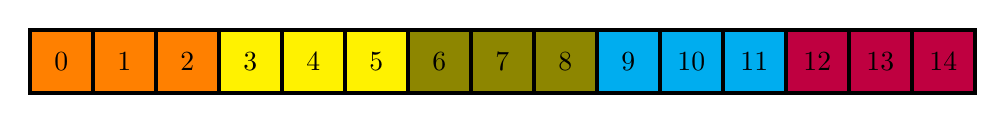
\begin{tikzpicture}[scale=0.8]
\draw [fill=orange,ultra thick] (0,0) rectangle (1,1);
\draw [fill=orange,ultra thick] (1,0) rectangle (2,1);
\draw [fill=orange,ultra thick] (2,0) rectangle (3,1);
\draw [fill=yellow,ultra thick] (3,0) rectangle (4,1);
\draw [fill=yellow,ultra thick] (4,0) rectangle (5,1);
\draw [fill=yellow,ultra thick] (5,0) rectangle (6,1);
\draw [fill=olive,ultra thick] (6,0) rectangle (7,1);
\draw [fill=olive,ultra thick] (7,0) rectangle (8,1);
\draw [fill=olive,ultra thick] (8,0) rectangle (9,1);
\draw [fill=cyan,ultra thick] (9,0) rectangle (10,1);
\draw [fill=cyan,ultra thick] (10,0) rectangle (11,1);
\draw [fill=cyan,ultra thick] (11,0) rectangle (12,1);
\draw [fill=purple,ultra thick] (12,0) rectangle (13,1);
\draw [fill=purple,ultra thick] (13,0) rectangle (14,1);
\draw [fill=purple,ultra thick] (14,0) rectangle (15,1);

\node at (0.5,.5) {0};
\node at (1.5,.5) {1};
\node at (2.5,.5) {2};
\node at (3.5,.5) {3};
\node at (4.5,.5) {4};
\node at (5.5,.5) {5};
\node at (6.5,.5) {6};
\node at (7.5,.5) {7};
\node at (8.5,.5) {8};
\node at (9.5,.5) {9};
\node at (10.5,.5) {10};
\node at (11.5,.5) {11};
\node at (12.5,.5) {12};
\node at (13.5,.5) {13};
\node at (14.5,.5) {14};
\end{tikzpicture}
\caption{Example of 15 agents divided in 5 communities, consisting of 3 agents each}
\label{fig:fixed vicinity}
\end{center}
\end{figure}